\section{Klasifikacija}
\label{sec:Klasifikacija}

Jedan od glavnih problema u \v{c}itavom skupu je veliki broj nedostaju\c'{}ih vrednosti za zanr. Stoga smo poku\v{s}ali da napravimo klasifikator koji \'c{}e klasifikovati instance sa nepoznatim vrednostima za \v{z}anr, treniran nad onim podacima gde su te informacije dostupne.

Prvi problem na koji smo nai\v{s}li su nestandarne vrednosti za \v{z}anr (videti poglavlje \ref{sec:Preprocesiranje}), stoga smo kori\v{s}\'c{}enjem jednostavnih transformacija izvukli slogove sa nedvosmislenom vredno\v{s}\'c{}u za \v{z}anr, a eliminisali one koji su za \v{z}anr imali vrednosti koje nisu bile od zna\v{c}aja za analizu (neki slogovi su imali vi\v{s}e razli\v{c}tih \v{z}anrova). Takodje smo neke sli\v{c}ne \v{z}anrove spojili u jedan, zarad jednostavnijeg rada (na primer \emph{jazz} i \emph{blues} se \v{c}esto pojavljuju zajedno ih ima smisla posmatrati kao jedan \v{z}anr).

Za predikciju vrednosti \v{z}anra smo koristili atribite \emph{loudness}, \emph{tempo} i \emph{mode}. Na\v{z}alost, iz njihove prostorne rasprostranjenosti se vidi da ne postoji jednostavni separator instanci raznih klasa - slika \ref{fig:ZanrKlasifikacija}. Odlu\v{c}ili smo da isprobamo \emph{KNN} algoritam u nadi da \'c{}e male grupe pesama istog \v{z}anra lepo klasifikovati bliske instance. O\v{c}ekivano, najbolji model koji smo dobili je imao preciznost od $52.65\%$. Na slici \ref{fig:KNNgreske} se mo\v{z}e videti kako se gre\v{s}ka menjala sa razli\v{c}itim vrednostima za parametar $k$.

\begin{figure}[H]
    \centering
    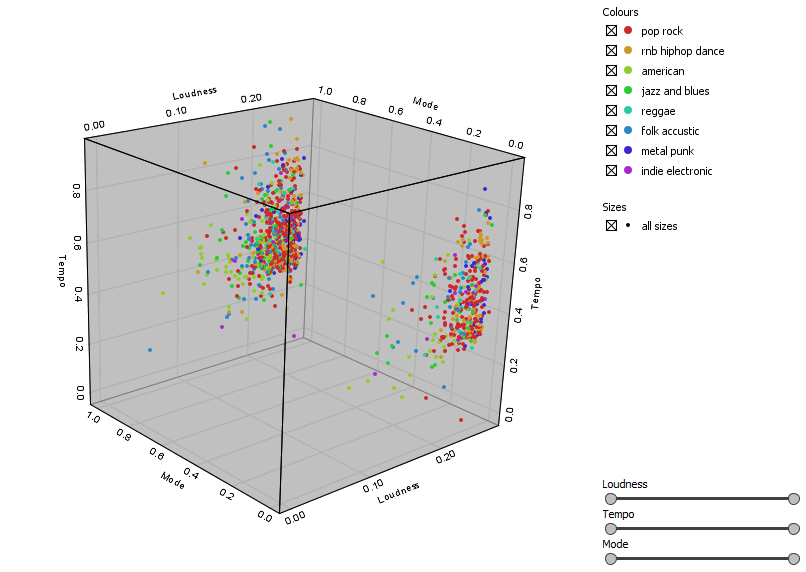
\includegraphics[scale=0.6]{resources/genre_scatter.PNG}
    \caption{3D prikaz pesama razli\v{c}itih \v{z}anrova u prostoru sa koordinatama \emph{loudness}, \emph{tempo} i \emph{mode}}
    \label{fig:ZanrKlasifikacija}
\end{figure}

\begin{figure}[H]
    \centering
    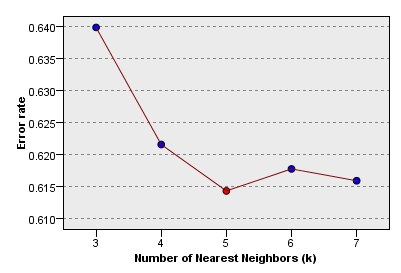
\includegraphics{resources/KNN_errors.PNG}
    \caption{Gre\v{s}ke dobijene za kreirane modele $k$ parametrom u opsegu $[3,7]$}
    \label{fig:KNNgreske}
\end{figure}

Ono \v{s}to nismo o\v{c}ekivali je jednaka va\v{z}nost atributa prilikom pravljenja klasifikatora - slika \ref{fig:KNNvaznost}. Intuicija nekako ka\v{z}e da su ja\v{c}e pesme podlo\v{z}nije da budu \v{z}anra \emph{metal}, ali rezultati su pobili tu intuiciju.

\begin{figure}[H]
    \centering
    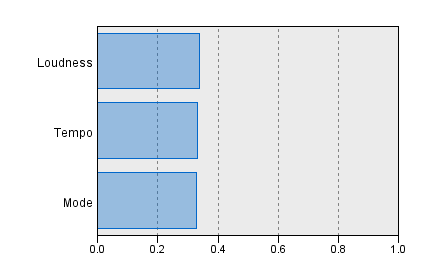
\includegraphics[scale=0.7]{resources/KNN_pred_imp.PNG}
    \caption{Va\v{z}nost atributa prilikom klasifikacije}
    \label{fig:KNNvaznost}
\end{figure}
